\section{Pipeline shell implementation}
\label{sec:pipelineShell}

The \textit{Pipeline shell} should be built on top of the ISS, simulating the timing of instructions through the pipeline, while the ISS simulates the functional execution of each instruction. This section will cover different approaches to modeling the pipeline shell.



\subsection{Full pipeline simulation}
\label{sec:fullPipeline}

The most accurate and complex simulation strategy is to simulate all the components of the pipeline, simulating all transitions, dependencies, stalls, etc, the same way the processor operates. This requires a tight coupling between the pipeline shell and the ISS, and it is necessary to split up the ISS into separate fetch, decode, execute, and writeback modules that are called from each corresponding stage from the pipeline shell. We also need to simulate all the intricacies of the pipeline, like hazards, forwarding, stalls, multi-cycle instructions, memory access, etc. 

This approach achieves very accurate results and fine-grained control over the behavior of the pipeline. However, this approach is challenging to implement and is very specialized to specific cores. Additionally, there is a risk of encountering the same bugs as the RTL implementation.

%
%We will detail what needs to be simulated for each pipeline stage below, using the CV32E40X as an example.
%
%\subsubsection{IF}
%The IF stage should simulate fetching the next instruction from memory. It should simulate memory access timing, pipeline stalls from cache misses, memory latency, etc. 
%
%
%\subsubsection{ID}
%
%To properly simulate the pipeline execution, we should simulate forwarding, dependencies, and hazards between instructions. Therefore, It is necessary to decode the instructions in this stage to extract the instruction type, registers, control signals, etc., necessary to calculate hazards. We should also read the values from the register file here to be used in the EX stage. In CV32E40X, jumps are taken from the ID stage and must also be simulated \cite{openhw_group_pipeline_2023}.
%
%\subsubsection{EX}
%
%In the EX stage, we must simulate all execution of instructions, including ALU, multiplication, and division. In the CV32E40X core, some instructions require multiple clock cycles to complete, so correct simulation of the EX stage requires stalling the EX stage for the correct number of clock cycles corresponding to the instruction type. Most instructions have a set number of clock cycles, while others have a variable amount. For instance, division and remainder operations can take between 3 and 35 cycles, depending on the operand value. This can be quite complicated and requires the simulator to simulate the division operation the same way as the core to get the correct amount of clock cycles. Alternatively, a simplified algorithm can be developed to determine the exact amount of clock cycles for a given operand.
%
%In addition, branches are taken from the EX stage, requiring calculation of the branch condition here. It must then take the branch, requiring a flush of IF and ID and a 3-4 cycle stall, or it must not take it.
%Additionally, the Load-Store-Unit (LSU) address generation and data requests are done in the EX stage.\cite{openhw_group_pipeline_2023}
%
%\subsubsection{WB}
%
%In the WB stage, the results are written to the correct registers. The second part of the LSU is also executed in the WB stage, so possible stalls from the LSU must be handled.
%
%In most Instruction Set Simulators (ISSs), the execution and write-back stages are combined into a single function. However, this approach can cause issues when using the execute function from the pipeline shell. The problem is that any changes made to the registers during this stage are immediately written back. As a result, it can lead to an inaccurate simulation if there are interruptions to program flow while in the EX stage that are finished in the ISS but then aborted in the actual implementation.\cite{openhw_group_pipeline_2023}
%
%We must modify the ISS to separate the execute and writeback functionality to solve this. This can be quite complicated as it changes fundamental parts of the operation of the ISS, and great care must be taken to ensure the ISS still operates correctly. Another solution could be to run the execute function in the writeback stage instead of the execute state. With this method, the effects of the instructions are correctly written back at the correct time. The disadvantage of this approach is that side effects from the execution will not be executed in the EX stage but in the WB stage. This could be solved with additional logic in the EX stage to execute these side effects in the EX stage.
%
%\subsubsection{Pipeline control}
%
%To properly model the pipeline, we need a module to determine when an instruction can advance to the next stage, considering stalls, multi-cycle operations, forwarding, data hazards, branch mispredictions, pipeline flushes, etc.
%
%
%\subsubsection{Interrupts}
%
%In this approach, the goal of accurately simulating the entire pipeline is for interrupts to be passed directly into the model at the correct time and for the model to simulate the handling correctly. 
%To determine when an interrupt can be taken, the model must check the contents of the pipeline stages and determine if all necessary conditions for an input to be taken are fulfilled. 
%If the interrupt can not be taken, it must halt the ID stage and continue executing instructions until all conditions apply.
%When the interrupt can be taken, it must flush the pipeline and load the interrupt handler correctly. \cite{openhw_group_exceptions_2023}

\subsection{Simplified Simulation} 


%In the following approach, we attempt to simplify the approach in \cref{sec:fullPipeline} by simulating only the essential components for correct verification of asynchronous events while abstracting away the rest.

To avoid unnecessary complexity, we only want to simulate the components necessary to verify asynchronous events properly while abstracting away the rest. Therefore, we propose the method below to find the optimal abstraction level of the pipeline shell.

\subsubsection{Finding the appropriate abstraction level}

\begin{enumerate}
    \item Find all requirements that affect the timing of interrupts.
    \item Analyze each requirement to identify the underlying requirements. 
    \item When all fundamental requirements are found, identify the necessary simulations to achieve each fundamental requirement, creating a dependency tree.
    \item Analyze the dependency tree to determine which abstractions can be done and which dependencies require accurate simulation.
\end{enumerate}

%\subsubsection{Simulation components}
%
%Components necessary to fully simulate the CV32E40X
%
%\begin{enumerate}
%    \item IF stage - Fetches 1 instruction per cycle, through an aligning prefetch buffer, if the memory allows.
%    \begin{itemize}
%        \item normal fetch
%        \item Bus error
%        \item Multiple outstanding memory transactions
%        \item Memory access delay
%        \item Misaligned accesses
%        \item stall - if instruction issued during single step
%    \end{itemize}
%    \item ID stage
%    \begin{itemize}
%        \item Instruction decoding
%        \item stalling - e.g. if pending interrupt 
%        \item Hazard if an instruction causing implicit CSR read in ID while csr access in WB
%        \item 2 cycle stall hazard if an instruction causing implicit CSR read in ID while csr access in WB
%        \item Jump happens from ID
%    \end{itemize}
%    \item EX stage
%    \begin{itemize}
%        \item Instruction execution
%        \item ALU, Multiplier, and Divider
%        \item Branches happen from EX if conditions are met
%        \item Stalls until multi-cycle instructions are complete. Multi-cycle instructions can be fixed or variable in length.
%        \item Address generation for Load-store-unit (LSU) is done in EX 
%    \end{itemize}
%    \item WB stage
%    \begin{itemize}
%        \item Write results back to register file
%        \item Second part of LSU. Takes one bus transaction for aligned and 2 misaligned transfers.
%        \item Simulate memory access delay 
%    \end{itemize}
%    \item Hazards
%    \item Stalls
%    \item Forwarding
%    \item Pipeline flushing
%    \item Branching
%    \item Jumps
%    \item CSR 
%    \item compressed instructions
%\end{enumerate}


To build a dependency tree for the CV32E40X core, we base the exploration on the RTL code in \cite{noauthor_openhw_2023}. From \lstinline{cv32e40x_controller_fsm.sv}, we can see that interrupts are taken if there is a pending interrupt and interrupt is allowed. Whether interrupts are allowed to be taken in CV32E40X depends on the following factors taken from the code:

\pagebreak

\begin{lstlisting}
  // Allow interrupts to be taken only if there is no data request in WB,
  // and no trans_valid has been clocked from EX to environment.
  // Not allowing interrupts when the core cannot take interrupts due to debug conditions.
  // Offloaded instructions in WB also block, as they cannot be killed after commit_kill=0 (EX stage)
  // LSU instructions which were suppressed due to previous exceptions or trigger match
  // will be interruptable as they were converted to NOP in ID stage.
  // When a fencei is present in WB and the LSU has completed all tranfers, the fencei handshake will be initiated. This must complete and the fencei instruction must retire before allowing interrupts.
  // Any multi operation instruction (table jumps, push/pop and double moves) may not be interrupted once the first operation has completed its operation in WB.
  //   - This is guarded with using the sequence_interruptible, which tracks sequence progress through the WB stage.
  // When a CLIC pointer is in the pipeline stages EX or WB, we must block interrupts.
  //   - Interrupt would otherwise kill the pointer and use the address of the pointer for mepc. A following mret would then return to the mtvt table, losing program progress. 
\end{lstlisting}

\begin{figure}[ht]
    \centering
    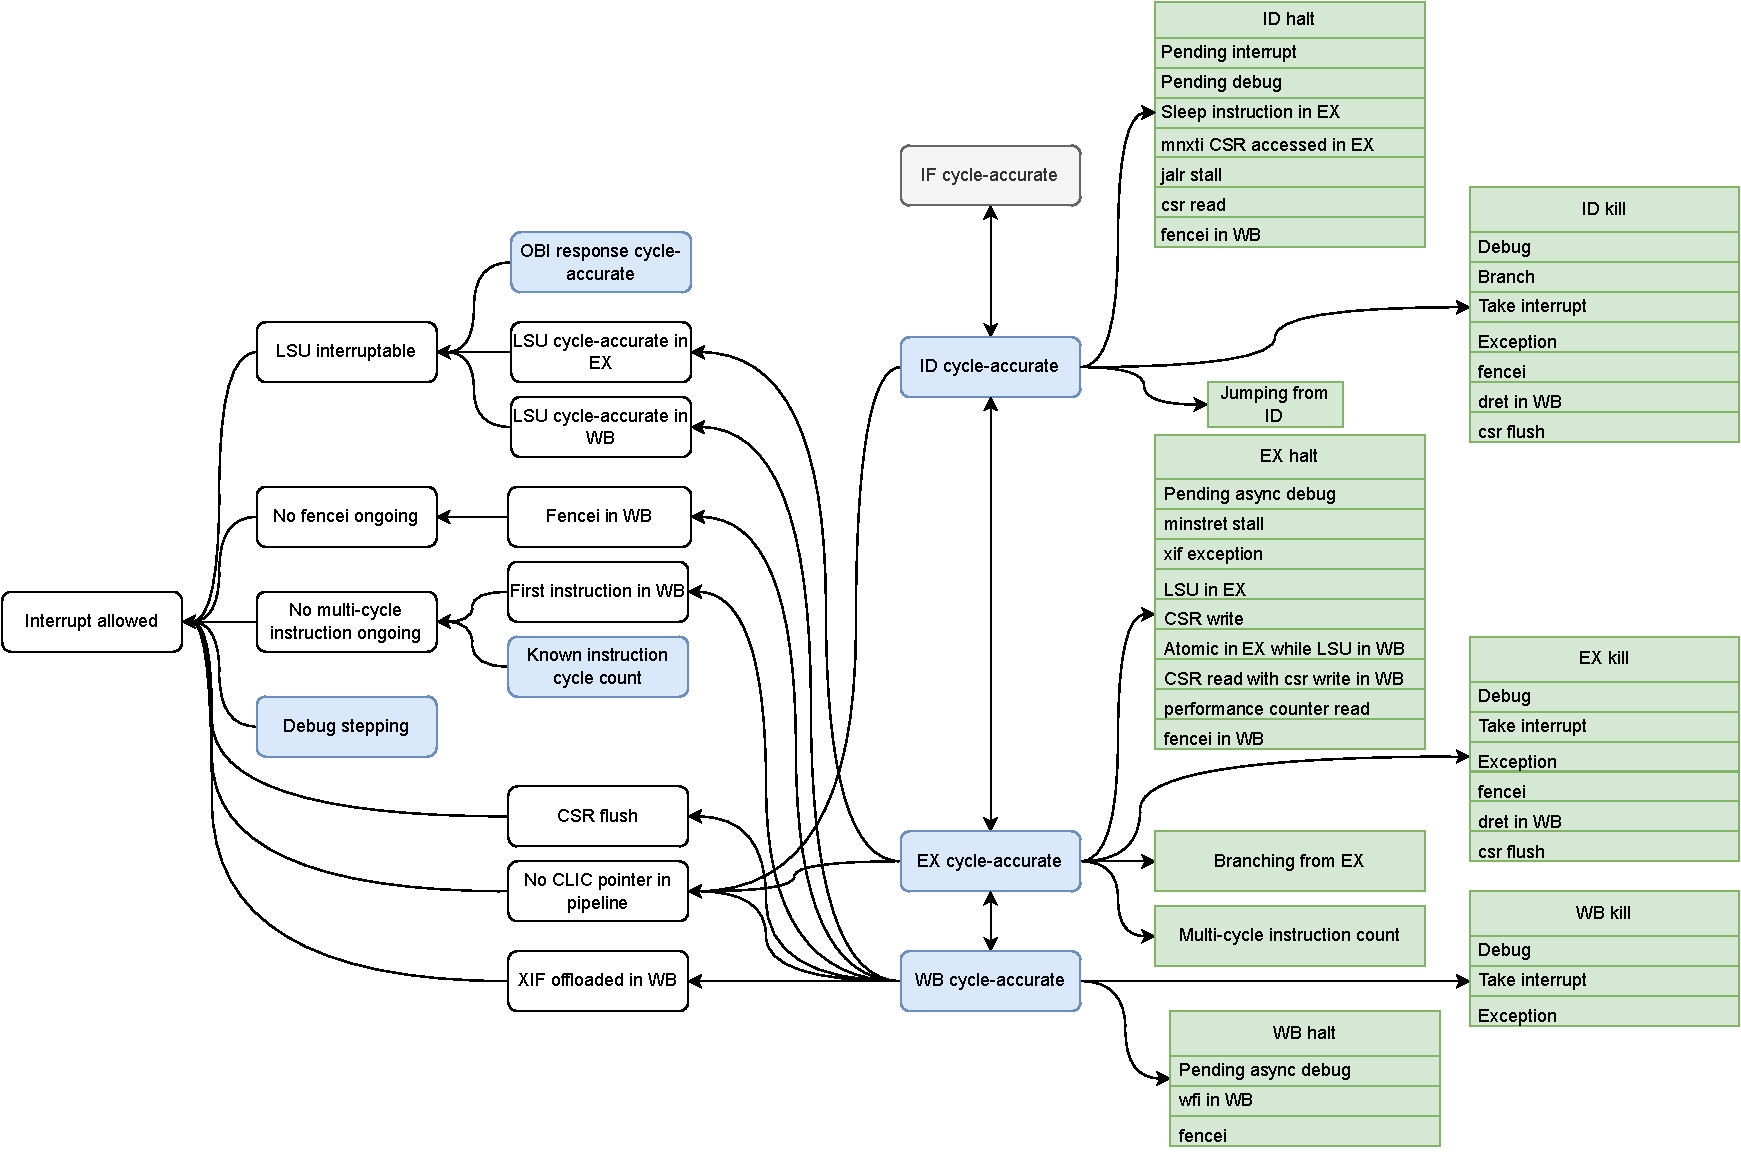
\includegraphics[width=1\linewidth]{pictures/Dependencies.pdf}
    \caption{Simulation dependency tree for interrupt handling in the CV32E40X core.}
    \label{fig:dependencyTree}
\end{figure}


We use this as a basis for building a dependency tree. The dependency tree is shown in \cref{fig:dependencyTree}. In the first layer, we see the following requirements:


\begin{itemize}
    \item The LSU is interruptable:
    %\begin{itemize}
    %    \item No data request in WB
    %    \item \lstinline{trans_valid} has not been clocked from EX
    %    \item The address phase is done, without finishing with \lstinline{resp_valid=1} in WB
    %    \item For misaligned split instructions, we may interrupt during the first cycle of the first half. If the first half stays in EX for more than one cycle, we cannot interrupt it (\lstinline{trans_valid_q == 1}). When the first half goes to WB, \lstinline{cnt_q != 0} will block interrupts. If the first half finishes in WB before the second half gets grant, \lstinline{trans_valid_q} will again be 1 and block interrupts, and \lstinline{cnt_q} will block the last half while it is in WB.
    %\end{itemize}
    \item When a fencei instruction is present in WB and the LSU has completed all tranfers, the fencei handshake will be initiated. This must complete and the fencei instruction must retire before allowing interrupts. 
    \item Don't allow interrupts in debug mode or single stepping without \lstinline{dcsr.stepie} set.
    \item Any multi-operation instruction may not be interrupted once the first operation has completed its operation in WB.
    \item Don't allow interrupts when a CLIC pointer is in the pipeline.
    \item Don't allow interrupts when a CSR flush happens
    \item Don't allow interrupts when an XIF instruction is offloaded in the WB.
    
\end{itemize}

From this, we can figure out what requirements are necessary. For the LSU to be interruptible, LSU instructions must be accurate in the EX and WB stage. We also need to know at which cycle the LSU gets a response via the OBI interface.
To know if a fencei transaction is in progress, we must know if the fencei instruction is in WB. To properly simulate multi-cycle instructions, we need to know when the first cycle has started by knowing if the first cycle is in WB, and we must know how many cycles the instruction will take. We must also know if we are in the debug mode, if there is a CLIC pointer in the pipeline, and if there is an offloaded XIF instruction in WB.

From these discoveries, we can deduce the fundamental requirements listed below, shown in blue in \cref{fig:dependencyTree}.
\begin{itemize}
    \item OBI response cycle-accurate
    \item Known instruction cycle count for multi-cycle instructions
    \item Debug stepping mode
    \item Instructions are cycle-accurate in the ID stage
    \item Instructions are cycle-accurate in the EX stage
    \item Instructions are cycle-accurate in the WB stage
\end{itemize}

From these requirements, we can determine what simulation components are necessary to accurately simulate the requirements above. These components are shown in green in \cref{fig:dependencyTree}. This shows that for each pipeline stage, we need to simulate halting and flushing of the stage, with all the requirements for halting and flushing shown in green. In addition, we must simulate jumping from the ID stage, branching from the EX stage, and accurate multi-cycle instruction execution in the EX stage.

\subsubsection{Abstractions}

From the dependency tree in \cref{fig:dependencyTree}, we can figure out what abstractions can be made and what functionality must be included. Further work should go into further analyzing what simplifications can be made and which implementation approaches can best fulfill these.

%\textbf{TODO: The important thing is that the order of instructions stay the same, and side effects happen at the correct time}

%RV32I has unconditional jumps and conditional branches. The control transfer instructions do not have architecturally visible delay slots\cite{waterman_risc-v_nodate}
%
%A UVM agent can be used to listen to the bus transactions from the DUT to synchronize when instructions are loaded into the core, when there is a cache miss etc.

%\subsection{Exploration of state changes (ImperasDV inspired) }
%
%\textbf{TODO: Further Discuss how the ImperasDV type functionality can be implemented}
%
%\subsubsection{Functionality required for this implementation}
%
%\begin{itemize}
%    \item Find all legal state transitions from the current state
%    \item Loop over all the sets of state transitions until retirement and check the result
%    \item Requires changing of state variables, executing an instruction, then undoing the changes, applying another state transition, and executing the instruction again.
%\end{itemize}
%
%\subsubsection{Using formal methods?}
%
%Could be used to find all legal state transitions, then go down each path, etc.
%
%Sail also generates models for formal methods
%

\subsection{Pipeline-shell implementation approaches}

This section will propose two approaches to modeling the pipeline shell.

\subsubsection{Stage-based pipeline simulation}
\label{sec:stagebased}

One approach to modeling the pipeline in a simulator is to use slots for each pipeline stage and move the instructions through the pipeline.
This can be done similarly to the approach used by the MARSS-RISCV explained in \cref{sec:marss}. As in MARSS-RISCV, we can use an object for each pipeline stage, holding an instruction object and info about the stage. A function corresponding to each stage can be used to move the instruction objects through the simulated pipeline. By running the functions in reverse order, we can ensure stalls are considered.

This approach provides a flexible and effective way of modeling the pipeline. We can also integrate the instruction data type from the ISS as the instruction placeholder to communicate with the ISS easily, or we can integrate an RVFI item for a specific instruction. Since the method closely resembles real-world behavior, it is also easier to understand, and stalls are easy to simulate.


\subsubsection{Cycle-based Time wheel simulation}
\label{sec:timeWheel}

Another approach is to model the simulator using a technique inspired by the timing shell from \cite{chiang_efficient_2009}, further explained in \cref{sec:cycle-accurate}. Instead of having slots for each pipeline stage, this approach has slots for each clock cycle, stored in a \textit{time wheel}. It has a \textit{commander} responsible for sending instructions to the ISS (or not in the case of a stall) and a scheduler that fills the slots in the time wheel with the correct state changes for that cycle. The scheduler is also the only component needing an in-depth understanding of the implementation details to place the state update correctly in the time wheel. 

This approach can get a little bit complicated when considering asynchronous events. When an interrupt is taken, and the pipeline must be flushed, the update corresponding to the different instructions might be spread out over different clock-cycle slots in the time wheel. This might make removing the changes corresponding to flushed instructions difficult while keeping unaffected instructions.


\begin{figure}[ht]
    \centering
    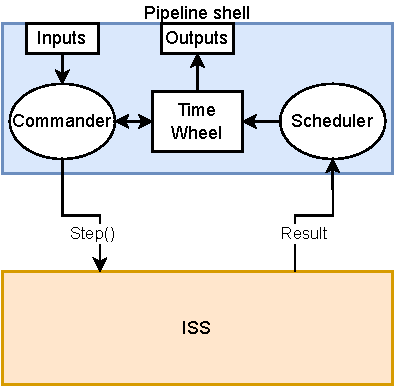
\includegraphics[width=0.5\linewidth]{pictures/time-wheel.pdf}
    \caption{Block diagram of pipeline shell with time wheel.}
    \label{fig:time-wheel}
\end{figure}


\subsection{Comparison}
\label{sec:stageWheelComp}

An important consideration is how the different approaches must be modeled to handle asynchronous events. In the time wheel approach, a single instruction and pipeline stage can have effects stored in multiple cycle slots. Additionally, a single cycle slot can also contain effects from multiple instructions. This can make it difficult to modify single stages or instructions, for instance, to flush a few pipeline stages when taking an interrupt.
On the other hand, the stage-based approach keeps the stage intact, allowing us to halt or flush selected stages more easily.

Another complication for the pipeline simulation is multicycle instructions. Using the CV32E40X core as an example, the longest instruction is the division operation and can last up to 35 cycles \cite{openhw_group_pipeline_2023}. To correctly model this in the time wheel approach, the scheduler needs to know the correct cycle count when inserting the instruction into the time wheel, and the time wheel must be large enough to hold all the cycles. In the stage-based design, this can be modeled by stalling the EX stage for the correct number of cycles, simplifying the design. 

Because the stage-based design follows the flow of the RTL pipeline, stalls can be easily modeled since the preceding pipeline stage can signal if it can be updated, and if not, the following stage must stall. In the time wheel approach, the scheduler must determine beforehand if stalls are necessary and insert these into the time wheel.

In summary, the stage-based approach might be the easiest approach to understand and implement, both for normal execution and for modifications due to asynchronous events. However, the different abstraction levels of the time wheel approach can be beneficial to avoid a simulator that too closely copies the core, implementing the same bugs in both. More work should go into further analyzing both, specifically determining how an asynchronous event can be modeled in both, as well as comparing the complexity details closely.





%\begin{table}[ht]
%\centering
%
%\begin{tabularx}{\textwidth}{|p{30mm}|*{2}{>{\arraybackslash} X |}}
%\hline
%\textbf{Feature}                     & \textbf{Stage-Based Pipeline Simulation}                                  & \textbf{Cycle-Based Time Wheel Simulation}                        \\ \hline
%\textbf{Representation}              & Models pipeline as a series of sequential stages                          & Organizes simulation around clock cycles                          \\ \hline
%\textbf{Intuitiveness}               & Mirrors real-world pipeline architecture, providing easy understanding    & Abstracts away pipeline details, making it less intuitive         \\ \hline
%\textbf{Efficiency}                  & Efficiently models instruction movement through pipeline                  & May require more complex data structures and algorithms           \\ \hline
%\textbf{Stall Simulation}            & Seamlessly simulates stalls                                               & May require additional logic for precise stall handling           \\ \hline
%\textbf{Asynchronous Event Handling} & Simpler to handle as stalls and flushing can be applied to specific stages             & Modifications to a stage, like a stall or flush, may be more complex since stages are represented in multiple cycle slots in the time wheel \\ \hline
%\textbf{Implementation Complexity}   & Generally simpler implementation due to direct representation of pipeline & May require more complex scheduling and state management \\ \hline
%\end{tabularx}
%\end{table}